\section{Graph-Vicinal Anchor Recovery}
\label{sec:method}

\begin{figure*}[t]
  \centering
  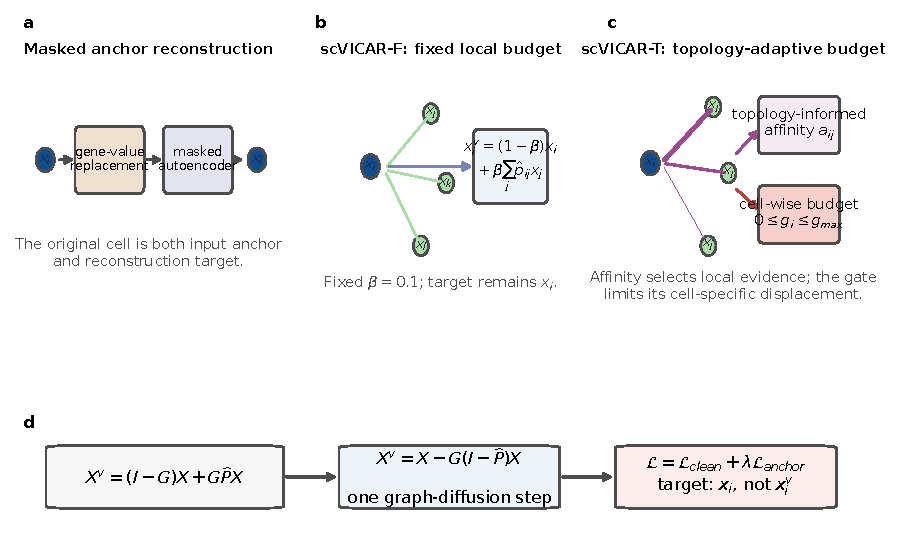
\includegraphics[width=\textwidth]{../figures/final/fig1_method.pdf}
  \caption{scVICAR framework. (a) The masked backbone reconstructs the original
  anchor. (b) scVICAR-F forms a bounded view with a fixed cell-wise budget and
  the cosine base kernel. (c) scVICAR-T augments the base kernel with analytic
  topology reliability and adapts the perturbation budget by cell. (d) Both
  variants are one-step graph-vicinal corruptions whose target remains the
  original anchor, rather than an interpolated label or target.}
  \label{fig:method}
\end{figure*}

Let $X=[x_1,\ldots,x_n]^\top\in\mathbb{R}^{n\times d}$ denote the
preprocessed expression matrix.  In the clean primary protocol, cell-type
labels are excluded from preprocessing choices, graph construction,
representation learning, and model selection.  They enter the preregistered
evaluation and explicitly separated downstream analyses.  The controlled
stress experiment is the sole graph-construction exception: labels deliberately
identify cross-class replacement edges after the clean protocol is frozen.
Figure~\ref{fig:method} summarizes the common anchor-recovery objective and the
fixed versus topology-adaptive corruption paths.

\subsection{Preprocessing and Matched Backbone}

For count-like input, we normalize each cell to a library size of $10^4$ and
apply $\log(1+x)$.  We then request 1,000 Seurat-style highly variable genes and
standardize each selected gene.  When fewer than 1,000 finite normalized
dispersions are available, a deterministic empirical-variance fallback enforces
exactly 1,000 genes; this prevents silent all-gene expansion.  Every comparison
in the matched-backbone study uses the
same three-layer encoder, mask predictor, linear decoder, optimizer, training
budget, and preprocessing.  The encoder maps $d$ genes through widths
$256\rightarrow128\rightarrow128$; a linear head predicts a $d$-dimensional
corruption mask, and the decoder reconstructs expression from the concatenated
latent vector and mask logits.

For a minibatch, let $M\in\{0,1\}^{b\times d}$ be a Bernoulli mask and let
$\Pi$ be one random permutation of the batch.  The scMAE corruption is
\begin{equation}
 C_{M,\Pi}(X_B)=(1-M)\odot X_B+M\odot\Pi X_B .
 \label{eq:scmae-corruption}
\end{equation}
Because a proposed replacement can equal the original value, the supervised
mask is the realized indicator
$\widetilde M=\mathbf{1}[C_{M,\Pi}(X_B)\neq X_B]$, rather than the initial
Bernoulli draw.  Given reconstruction $\widetilde X$ and predicted mask logits
$U$, the per-cell backbone loss is
\begin{align}
 \ell_i^{\mathrm{MAE}}
 &= (1-\lambda_m)\frac{1}{d}\sum_{r=1}^d
 w_{ir}(\widetilde x_{ir}-x_{ir})^2
 \nonumber\\
 &\quad+\lambda_m\frac{1}{d}\sum_{r=1}^d
 \operatorname{BCELogit}(u_{ir},\widetilde m_{ir}),
 \label{eq:backbone-loss}\\
 w_{ir}&=\lambda_x\widetilde m_{ir}+(1-\lambda_x)(1-\widetilde m_{ir}).
\end{align}
Protocol v1 fixes $\lambda_x=0.75$ and $\lambda_m=0.7$.

\subsection{Static Cell Graph}

We compute a 50-dimensional PCA representation, normalize its rows to unit
length, and construct a directed cosine $k$-nearest-neighbor graph with $k=5$.
For $j\in\mathcal N_i$, let $s_{ij}$ be cosine similarity and
$d_{ij}=1-s_{ij}$.  The base transition probability is
\begin{equation}
 p_{ij}^{(0)}=
 \frac{\exp(s_{ij}/\tau)}{\sum_{\ell\in\mathcal N_i}\exp(s_{i\ell}/\tau)},
 \qquad \tau=0.2.
 \label{eq:base-kernel}
\end{equation}
The graph is constructed once before training; scVICAR does not dynamically
update it from the learned representation.

The implementation samples $m=4$ neighbor positions with replacement.  If
$J_{ir}\sim\operatorname{Categorical}(q_i)$, the realized row-stochastic kernel
is
\begin{equation}
 \widehat p_{ij}=
 \frac{\sum_{r=1}^{m}\mathbf{1}[J_{ir}=j]q_{ij}}
 {\sum_{r=1}^{m}q_{iJ_{ir}}}.
 \label{eq:realized-kernel}
\end{equation}
This definition is deliberately faithful to the sampling-then-reweighting
estimator: it is not presented as an unbiased estimator of
$\sum_jq_{ij}x_j$.  The unbiased random average and full-neighborhood
aggregation are evaluated only as mechanism ablations.

\subsection{scVICAR-F: Fixed Vicinal Corruption}

For each anchor cell, the neighborhood aggregate is
$\bar x_i=\sum_j\widehat p_{ij}x_j$.  scVICAR-F forms
\begin{equation}
 x_i^v=(1-g)x_i+g\bar x_i,
 \qquad g=0.1,
 \label{eq:fixed-view}
\end{equation}
which corresponds to the original NeighborMix coefficient $\alpha=1-g=0.9$.
Crucially, $x_i^v$ is an input view rather than a synthetic biological target.
After applying the same corruption mechanism in Eq.~\eqref{eq:scmae-corruption}
with an independent mask and batch-permutation draw for this branch, the decoder
is trained to recover the original anchor $x_i$.  We therefore call the
objective \emph{graph-vicinal anchor recovery}, distinguishing it from mixup,
which interpolates inputs and supervision together~\cite{zhang2018mixup}.

\subsection{scVICAR-T: Topology-Adaptive Corruption}

scVICAR-F already uses the nonuniform cosine-softmax base kernel
$p_{ij}^{(0)}$, including the implemented sampling-then-reweighting estimator,
but applies the same gate to every anchor and no mutual-KNN or SNN reliability
correction.  scVICAR-T adds those topology corrections and a cell-wise
perturbation budget.  Let $m_{ij}$ indicate a mutual-KNN relation, and let
\begin{equation}
 q_{ij}^{\mathrm{SNN}}=
 \frac{|\mathcal N_i\cap\mathcal N_j|}
 {|\mathcal N_i\cup\mathcal N_j|}
\end{equation}
be shared-nearest-neighbor overlap.  The unnormalized topology-informed
affinity is
\begin{equation}
 a_{ij}\propto p_{ij}^{(0)}
 e^{\gamma_s s_{ij}}
 (1+\gamma_m m_{ij})
 (1+\gamma_q q_{ij}^{\mathrm{SNN}})
 e^{-\gamma_d d_{ij}},
 \label{eq:topology-affinity}
\end{equation}
normalized across $\mathcal N_i$.  In Eq.~\eqref{eq:realized-kernel}, scVICAR-F
uses $q_i=p_i^{(0)}$, whereas scVICAR-T uses $q_i=a_i$.

The cell-wise gate uses mutual-neighbor ratio, mean SNN overlap, and a
similarity-weighted perturbation proxy:
\begin{align}
 \bar m_i&=k^{-1}\sum_{j\in\mathcal N_i}m_{ij},\\
 \bar q_i&=k^{-1}\sum_{j\in\mathcal N_i}q_{ij}^{\mathrm{SNN}},\\
 \rho_i&=1-\sum_{j\in\mathcal N_i}p_{ij}^{(0)}s_{ij},\\
 g_i&=g_{\min}+(g_{\max}-g_{\min})
 \sigma(\beta_m\bar m_i+\beta_q\bar q_i-\beta_\rho\rho_i).
 \label{eq:topology-gate}
\end{align}
Protocol v1 sets $g_{\min}=0$, $g_{\max}=0.1$,
$\beta_m=\beta_q=1$, and $\beta_\rho=2$.  No uncertainty estimate, learned
gate, clustering assignment, label, or dynamic graph enters this expression.

\subsection{Unified Objective and Inference}

Let $G=\operatorname{diag}(g_1,\ldots,g_n)$.  Both variants take the unified
form
\begin{equation}
 X^v=(I-G)X+G\widehat P X
     =X-G(I-\widehat P)X .
 \label{eq:unified-view}
\end{equation}
scVICAR-F has $G=0.1I$; scVICAR-T uses Eq.~\eqref{eq:topology-gate}.  For a
minibatch $B$, the adaptive vicinal loss uses
$\omega_i=g_i/\max_{\ell\in B}g_\ell$ and
\begin{align}
 \mathcal L_B
 &=\frac{1}{|B|}\sum_{i\in B}\ell_i^{\mathrm{MAE}}(x_i)\nonumber\\
 &\quad+\lambda_v
 \frac{\sum_{i\in B}\omega_i\ell_i^{\mathrm{MAE}}(x_i^v\!\rightarrow x_i)}
 {\sum_{i\in B}\omega_i},\qquad \lambda_v=0.3.
 \label{eq:objective}
\end{align}
The fixed variant has uniform nonzero weights.  The preregistered model uses no
contrastive or explicit embedding-consistency term.  At inference, the clean
matrix is passed through the encoder without graph propagation.  Clustering is
performed afterward and is not part of the representation-learning objective.

All matched variants use 80 epochs, batch size 256, learning rate $10^{-3}$,
mask ratio 0.4, a 128-dimensional embedding, and identical random seeds.  The
NoMix control sets $G=0$ and $\lambda_v=0$; edge-only and gate-only variants
isolate the two adaptive components, and random mixing controls for generic
convex perturbation without local geometry.
